\section{O papel do analisador sintático}

\begin{frame}[fragile]{Gramáticas no projeto de linguagens e na escrita de compiladores}

    \begin{itemize}
        \item Uma gramática oferece uma especificação sintática precisa para uma linguagem de programação
        \pause

        \item Para certas classes de gramática é possível gerar o analisador sintático automaticamente
        \pause

        \item O processo de construção do analisador sintático permite identificar ambiguidades sintáticas e outras construções difíceis de analisar, ajudando o
            projeto inicial de uma linguagem
        \pause

        \item Uma gramática bem projetada implica uma estrutura para a linguagem que é útil para a tradução para a linguagem alvo e para a detecção de erros
        \pause

        \item A inclusão de novas características em uma linguagem é facilitada se a implementação foi baseada em uma descrição gramatical
    \end{itemize}

\end{frame}

\begin{frame}[fragile]{O papel do analisador sintático}

    \begin{itemize}
        \item O analisador sintático recebe, do analisador léxico, uma cadeia de \textit{tokens} e verifica se esta cadeia pode ser gerada pela gramática da
            linguagem-fonte
        \pause

        \item Ele também deve relatar quaisquer erros de sintaxe que possam surgir, de forma inteligível
        \pause

        \item Se possível, ele deve se recuperar dos erros mais comuns
        \pause

        \item Ele pode produzir, explicitamente ou implicitamente, uma árvore sintática 
    \end{itemize}

\end{frame}

\begin{frame}[fragile]{Posição do analisador sintático num modelo de compilador}

    \begin{figure}
        \centering 

        \begin{scriptsize}
        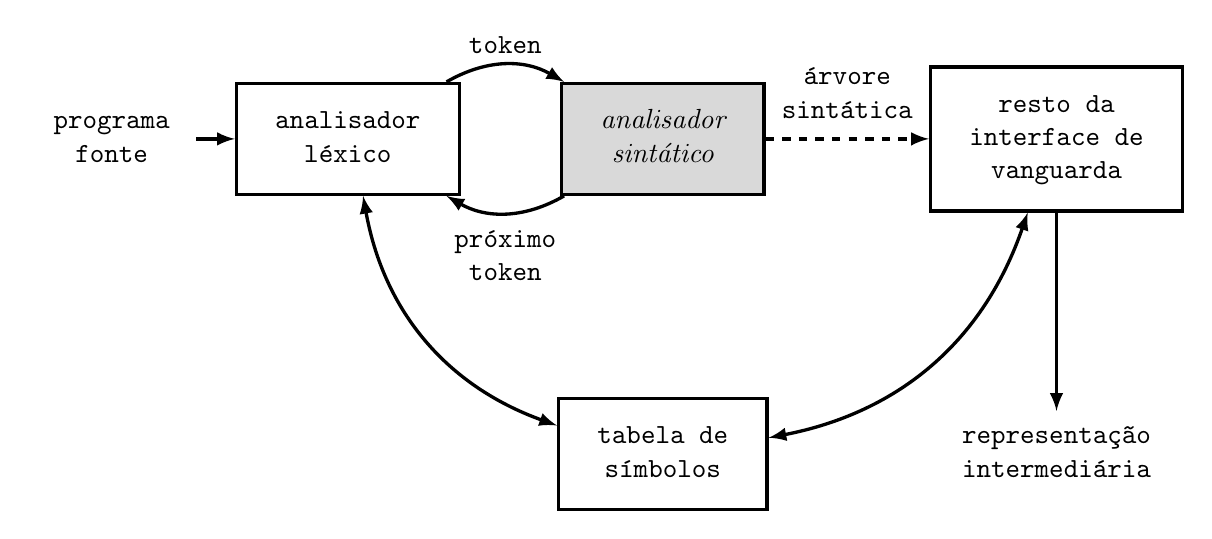
\begin{tikzpicture}
            \node (A) at (0, 6) { \texttt{\begin{tabular}{c}programa\\ fonte\end{tabular}} };
            \node[draw,very thick,inner sep=8pt] (B) at (3, 6) { \texttt{\begin{tabular}{c}analisador\\ léxico\end{tabular}} };
            \node[draw,very thick,inner sep=8pt,fill=gray!30] (C) at (7, 6) { \textit{\begin{tabular}{c}analisador\\ sintático\end{tabular}} };
            \node[draw,very thick,inner sep=8pt] (D) at (7, 2) { \texttt{\begin{tabular}{c}tabela de\\ símbolos\end{tabular}} };
            \node[draw,very thick,inner sep=8pt] (E) at (12, 6) { \texttt{\begin{tabular}{c}resto da\\ interface de\\ vanguarda\end{tabular}} };
            \node (F) at (12, 2) { \texttt{\begin{tabular}{c}representação\\ intermediária\end{tabular}} };

            \draw[very thick,-latex] (A) to (B);
            \draw[very thick,-latex] (B) to [bend left] node[above] { \texttt{token}} (C);
            \draw[very thick,-latex] (C) to [bend left] node[below] { \texttt{\begin{tabular}{c}próximo\\ token\end{tabular}}} (B);
            \draw[very thick,-latex,dashed] (C) to node[above] { \texttt{\begin{tabular}{c}árvore\\ sintática\end{tabular}} } (E);
            \draw[very thick,latex-latex] (B) to [bend right] (D);
            \draw[very thick,latex-latex] (E) to [bend left] (D);
            \draw[very thick,-latex] (E) to (F);
        \end{tikzpicture}
        \end{scriptsize}
    \end{figure}

\end{frame}

\begin{frame}[fragile]{Tipos de analisadores sintáticos}

    \begin{itemize}
        \item Há três tipos gerais de analisadores sintáticos
        \pause

        \item O primeiro tipo são os métodos universais, que podem tratar quaisquer gramáticas
        \pause

        \item Exemplos de métodos gerais: o algoritmo de Younger-Kasami e o algoritmo de Early
        \pause

        \item Tais métodos são ineficientes para um compilador de produção
        \pause

        \item Os outros dois tipos são os analisadores \textit{top-down} e os analisadores \textit{bottom-up}
        \pause

        \item Estes métodos trabalham apenas com uma determinada subclasse de gramáticas, porém são mais eficientes que os métodos universais
    \end{itemize}

\end{frame}

\begin{frame}[fragile]{Tratamento dos erros de sintaxe}

    \begin{itemize}
        \item 
    \end{itemize}

\end{frame}
